\documentclass[crop, tikz]{standalone}
\usepackage{tikz}
\usetikzlibrary{patterns}


\definecolor{CBOrange}{HTML}{E69F00}
\definecolor{CBSkyBlue}{HTML}{56B4E9}
\definecolor{CBBlue}{HTML}{0072B2}
\definecolor{CBGreen}{HTML}{009E73}
\definecolor{CBYellow}{HTML}{F0E442}
\definecolor{CBRed}{HTML}{D55E00}
\definecolor{CBPurple}{HTML}{CC79A7}

\definecolor{foreground}{RGB}{255,255,255}
\definecolor{background}{RGB}{44,44,44}
\definecolor{lightbackground}{RGB}{60,60,60}



\usetikzlibrary{positioning}

\begin{document}
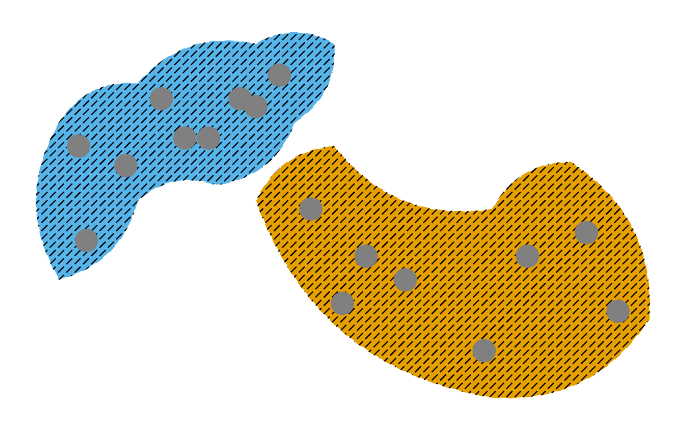
\begin{tikzpicture}
  
  \draw[foreground, dashed, fill=CBOrange, postaction={ pattern=north east lines  }] 
	  (4,0) to[bend right] (7,-2.5) to[bend right] (9,-1.5) to[bend right] (8,0.5) to[bend right] (7,-0.1) to[bend left] (5,0.7) to[bend right] (4,0);
	  
	 \draw[foreground, dashed, fill=CBSkyBlue, postaction={ pattern=north east lines  }]
	(1.5,-1) to[bend right] (2.5,0.0) to[bend left] (3.5,0.2) to[bend right] (4.5,1.0) to[bend right] (5,2) to[bend right] (4,2) to[bend right] (2.5,1.5) to[bend right] (1.5,1) to[bend right] (1.5,-1) ;	
	%\draw[ultra thick, gray, dashed] (5.5, 2) -- (5.5, -2);
	%\node[circle,inner sep=0.3em,fill=CBOrange,very thick] (X) at (4.5, 0.5) {};
	\node[circle,inner sep=0.3em,fill=gray,very thick] (Y) at (4.7, -0.1) {};
	%\node[circle,inner sep=0.3em,fill=CBOrange,very thick] (Y) at (5.2, 0.1) {};
	\node[circle,inner sep=0.3em,fill=gray,very thick] (Y) at (5.1, -1.3) {};
	%\node[circle,inner sep=0.3em,fill=CBOrange,very thick] (Y) at (5.6, -0.33) {};
	\node[circle,inner sep=0.3em,fill=gray,very thick] (Y) at (5.4, -0.7) {};
	%\node[circle,inner sep=0.3em,fill=CBOrange,very thick] (Y) at (5.8, -0.9) {};
	\node[circle,inner sep=0.3em,fill=gray,very thick] (Y) at (5.9, -1.0) {};
	%\node[circle,inner sep=0.3em,fill=CBOrange,very thick] (Y) at (6.4, -1.2) {};
	\node[circle,inner sep=0.3em,fill=gray,very thick] (Y) at (6.9, -1.9) {};
	%\node[circle,inner sep=0.3em,fill=CBOrange,very thick] (Y) at (7.4, -1.3) {};
	\node[circle,inner sep=0.3em,fill=gray,very thick] (Y) at (7.45, -0.7) {};
	%\node[circle,inner sep=0.3em,fill=CBOrange,very thick] (Y) at (7.8, -1.5) {};
	\node[circle,inner sep=0.3em,fill=gray,very thick] (Y) at (8.2, -0.4) {};
	%\node[circle,inner sep=0.3em,fill=CBOrange,very thick] (Y) at (8.3, -1.0) {};
	\node[circle,inner sep=0.3em,fill=gray,very thick] (Y) at (8.6, -1.4) {};
	
	

	
	%\node[circle,inner sep=0.3em,fill=CBSkyBlue,very thick] (Y) at (6.5, 0.5) {};
	\node[circle,inner sep=0.3em,fill=gray,very thick] (Y) at (3.1, 0.8) {};
	%\node[circle,inner sep=0.3em,fill=CBSkyBlue,very thick] (Y) at (5.7, 0.9) {};
	\node[circle,inner sep=0.3em,fill=gray,very thick] (Y) at (2.8, 1.3) {};
	%\node[circle,inner sep=0.3em,fill=CBSkyBlue,very thick] (Y) at (5.4, 1.15) {};
	\node[circle,inner sep=0.3em,fill=gray,very thick] (Y) at (4, 1.2) {};
	%\node[circle,inner sep=0.3em,fill=CBSkyBlue,very thick] (Y) at (4.8, 1.5) {};
	\node[circle,inner sep=0.3em,fill=gray,very thick] (Y) at (4.3, 1.6) {};
	%\node[circle,inner sep=0.3em,fill=CBSkyBlue,very thick] (Y) at (4.2, 1.2) {};
	\node[circle,inner sep=0.3em,fill=gray,very thick] (Y) at (3.8, 1.3) {};
	%\node[circle,inner sep=0.3em,fill=CBSkyBlue,very thick] (Y) at (3.4, 1.3) {};
	\node[circle,inner sep=0.3em,fill=gray,very thick] (Y) at (3.4, 0.8) {};
	%\node[circle,inner sep=0.3em,fill=CBSkyBlue,very thick] (Y) at (3.1, 1.1) {};
	\node[circle,inner sep=0.3em,fill=gray,very thick] (Y) at (1.75, 0.7) {};
	%\node[circle,inner sep=0.3em,fill=CBSkyBlue,very thick] (Y) at (2.45, 0.1) {};
	\node[circle,inner sep=0.3em,fill=gray,very thick] (Y) at (2.35, 0.45) {};
	%\node[circle,inner sep=0.3em,fill=CBSkyBlue,very thick] (Y) at (1.9, -0.04) {};
	\node[circle,inner sep=0.3em,fill=gray,very thick] (Y) at (1.85, -0.5) {};
	
    
\end{tikzpicture}
\end{document}